\section{Introduction}

\begin{frame}{Overview}
  \begin{itemize}
    \item Problem \& Motivation
    \item Related works
    \item Background concepts
    \item Method 1: Query2Label (Q2L)
    \item Method 2: Multi-label Learning from Single Positive Labels (MLSPL)
    \item Experiments 
    \item Results \& Discussion
    \item Conclusion
  \end{itemize}
\end{frame}
%-------------------------------------------------

\begin{frame}{Problem \& Motivation}
    \textbf{What is Multi-label Classification?}
  \begin{itemize}
    \item Assigns multiple labels to a single instance (e.g., an image with both “dog” and “cat”).
    \item  Unlike single-label (one label per image) or multi-class (choose one among many), multi-label allows overlapping labels.
  \end{itemize}

      \vfill
    \begin{figure}[b]
        \centering
        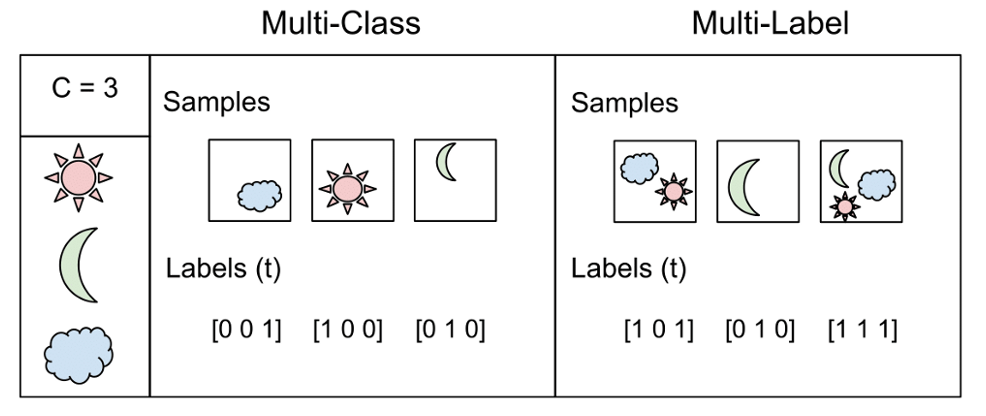
\includegraphics[width=0.8\linewidth]{Images/mlc.png}
        \caption*{\tiny Illustration of single-label vs multi-class vs multi-label classification. 
        From \url{https://medium.com/@wongsirikuln/fire-alert-system-with-multi-label-classification-model-explained-by-gradcam-bc18affe178c}.}
    \end{figure}
\end{frame}

\begin{frame}{Problem \& Motivation}
    \textbf{Applications}
  \begin{itemize}
    \item Image tagging 
    \item Medical imaging
    \item Autonomous driving
    \item Etc.
  \end{itemize}
\end{frame}

\begin{frame}{Problem \& Motivation}
  \textbf{Challenges}  
      \begin{itemize}
        \item Small objects and background clutter (feature recognition).
        \item Severe class imbalance.
        \item Growing annotation cost.
        \item Sparse annotations.
      \end{itemize}
\end{frame}

%-------------------------------------------------

\begin{frame}{Problem \& Motivation}
    \textbf{Project goals}
  \begin{itemize}
    \item Implemented two approaches: \\ \textbf{Q2L} and \textbf{MLSPL}.
    \item Reproduce results on MS-COCO 2014.
    \item Analyze resource trade-offs and reproducibility.
  \end{itemize}
\end{frame}

%-------------------------------------------------

\begin{frame}{Related work}
  \begin{itemize}
    \item Loss functions
    \item Locating areas of interest
    \item PU Learning
    \item Partially observed labels
    \item Attention and Transformer architectures
  \end{itemize}
\end{frame}